\section{Exact equivalence and equal-budget block sensitivity}
MARDM's~\cite{mardm2025} additive/replacement noise experiment compares its essential and redundant feature groups. For HumanML3D, these have 67 and 196 dimensions: root/local positions versus 126 rotation, 66 velocity and four contact values. Noise in the redundant group need not preserve represented rotations. The checked arXiv revision includes Appendices A--G but does not specify the Table 3 noise amplitude there. Our test addresses a different question with explicit per-clip total norm: how do equal-budget interventions inside and outside the rotation equivalence class affect the same frozen readers?

We use all twenty saved real-motion cohorts, each with 4,640 native entries and unchanged captions, crop lengths, masks and 32-candidate groups. For reader $r$ with its fixed native standard deviations $D_r$, the budget is
\begin{equation}
\left\|D_r^{-1}(y-x)\right\|_2=\kappa\sqrt L,\qquad\kappa\in\{1,3\}.
\end{equation}
The norm sums all valid frames and all 263 feature coordinates before feature selection, and is matched separately for every clip. Normalizers differ across readers, so a numerical radius is not interchangeable between T2M and TMR. Matching per-coordinate noise variance instead would allocate different total norm to blocks of different dimensions.

\paragraph{Interventions.}
Three null conditions use positive scales and shear: fixed coefficient directions $(1,-1,1)$ and its negative, and independent Gaussian coefficient directions per joint/frame. A per-clip scalar is solved from the input-space norm without evaluator scores. The rotation control uses independent isotropic axes, local SO(3) changes and canonical 6D output; its angle is solved from the same norm, with a maximum of $\pi/2$. Other block-only controls add Gaussian fields to velocities 193:259, contacts 259:263 and positions 4:67, holding root channels and all remaining blocks fixed. Registered seeds share fields across radii; padding and protected channels are restored bitwise.

the T2M evaluator's native movement encoder drops contacts, so its consumed contact budget is zero. This is a feature-selection negative control, not evidence that its learned weights ignore a consumed input. TMR reads all 263 dimensions. Continuous contact perturbations may leave the binary domain; other non-null controls can be inconsistent with unchanged blocks. These are feature-input ablations, not coherent physical-motion perturbations. The separate angular calibration jointly updates the relevant feature blocks.

\begin{table*}[t]
\centering\small
\caption{\textbf{All equal-L2 endpoints.} Twenty paired draws of 4,640 entries, two preselected radii, and seven interventions. Fourth/fifth columns are T2M FID or TMR matched-cosine change, respectively; R1 is a fraction. Intervals adjust 28 endpoints per reader. The T2M contact control has zero consumed budget; non-null controls need not be physically consistent across blocks.}\label{tab:matchedfull}
\begin{tabular}{@{}rllrrrr@{}}\toprule
Reader&$\kappa$&Intervention&$\Delta$ FID/cos&95\% interval&$\Delta$ R1&95\% interval\\\midrule
T2M&1&Null: fixed +&+0.006941&$[+0.006920,+0.006962]$&+0.000776&$[-0.000838,+0.002390]$\\
T2M&1&Null: fixed $-$&+0.007829&$[+0.007806,+0.007853]$&-0.001584&$[-0.003605,+0.000437]$\\
T2M&1&Null: random&+0.000045&$[+0.000042,+0.000047]$&-0.000162&$[-0.001152,+0.000829]$\\
T2M&1&Changed rotations&+0.000059&$[+0.000056,+0.000061]$&+0.000216&$[-0.000777,+0.001208]$\\
T2M&1&Velocities&+0.000179&$[+0.000170,+0.000187]$&+0.000226&$[-0.000912,+0.001365]$\\
T2M&1&Contacts&+0.000000&$[+0.000000,+0.000000]$&+0.000000&$[+0.000000,+0.000000]$\\
T2M&1&Positions&+0.000216&$[+0.000204,+0.000228]$&+0.000485&$[-0.000473,+0.001443]$\\
T2M&3&Null: fixed +&+0.082295&$[+0.082094,+0.082497]$&-0.001627&$[-0.004837,+0.001582]$\\
T2M&3&Null: fixed $-$&+0.116879&$[+0.116596,+0.117162]$&-0.010172&$[-0.013093,-0.007252]$\\
T2M&3&Null: random&+0.002379&$[+0.002318,+0.002440]$&-0.001897&$[-0.003738,-0.000055]$\\
T2M&3&Changed rotations&+0.003494&$[+0.003424,+0.003565]$&+0.000366&$[-0.001264,+0.001996]$\\
T2M&3&Velocities&+0.015856&$[+0.015569,+0.016142]$&-0.000226&$[-0.002694,+0.002242]$\\
T2M&3&Contacts&+0.000000&$[+0.000000,+0.000000]$&+0.000000&$[+0.000000,+0.000000]$\\
T2M&3&Positions&+0.018261&$[+0.017840,+0.018681]$&-0.000291&$[-0.002118,+0.001537]$\\
TMR&1&Null: fixed +&-0.000178&$[-0.000257,-0.000098]$&+0.000075&$[-0.000934,+0.001085]$\\
TMR&1&Null: fixed $-$&-0.000882&$[-0.000964,-0.000800]$&-0.000172&$[-0.001331,+0.000986]$\\
TMR&1&Null: random&+0.000061&$[+0.000045,+0.000076]$&+0.000086&$[-0.000572,+0.000744]$\\
TMR&1&Changed rotations&+0.000101&$[+0.000086,+0.000117]$&+0.000119&$[-0.000281,+0.000518]$\\
TMR&1&Velocities&+0.000020&$[+0.000005,+0.000034]$&-0.000011&$[-0.000615,+0.000594]$\\
TMR&1&Contacts&+0.000075&$[+0.000042,+0.000108]$&+0.000011&$[-0.000809,+0.000830]$\\
TMR&1&Positions&+0.000094&$[+0.000062,+0.000125]$&+0.000183&$[-0.000371,+0.000737]$\\
TMR&3&Null: fixed +&-0.003533&$[-0.003767,-0.003298]$&-0.001002&$[-0.002332,+0.000328]$\\
TMR&3&Null: fixed $-$&-0.006272&$[-0.006527,-0.006017]$&-0.002317&$[-0.003955,-0.000678]$\\
TMR&3&Null: random&+0.000514&$[+0.000459,+0.000569]$&+0.000108&$[-0.000956,+0.001172]$\\
TMR&3&Changed rotations&+0.000850&$[+0.000801,+0.000899]$&+0.000226&$[-0.000565,+0.001018]$\\
TMR&3&Velocities&+0.000036&$[-0.000028,+0.000099]$&-0.000011&$[-0.001178,+0.001157]$\\
TMR&3&Contacts&-0.001220&$[-0.001353,-0.001088]$&-0.002349&$[-0.004083,-0.000615]$\\
TMR&3&Positions&+0.000700&$[+0.000604,+0.000795]$&+0.000302&$[-0.000835,+0.001439]$\\
\bottomrule\end{tabular}\end{table*}

\paragraph{Endpoints and uncertainty.}
T2M reports FID against the same original real cohort, R1 and MM-distance; TMR reports native cosine retrieval and matched cosine. Paired-reference T2M FID has a zero baseline by construction. Twenty-draw paired $t_{19}$ intervals adjust 28 primary endpoints per reader, covering seven conditions, two radii and two scores. Null recodings additionally pass through canonicalization; their embedding and score closure is a numerical diagnostic. Fixed signs, random controls and both radii remain reported. Equal norm does not equalize physical information, direction, temporal coherence or neural sensitivity.

\paragraph{Independent verification.}
Every output's norm is checked during production. Independent checks recompute every saved metric and adjusted interval, check all per-clip norm arrays, and reconstruct the first eight raw fixtures of every condition/draw using separate formulas and SciPy rotations. They compare norms, represented matrices, native forward embeddings, protected channels and padding. Null conditions additionally receive one native FK pair per condition/draw. The checks do not claim a complete native geometry replay of unsaved arrays; protocols and scalar/seed records permit their reconstruction.

\section{Natural rotation deviations and model-family mechanism}
\begin{figure}[t]\centering
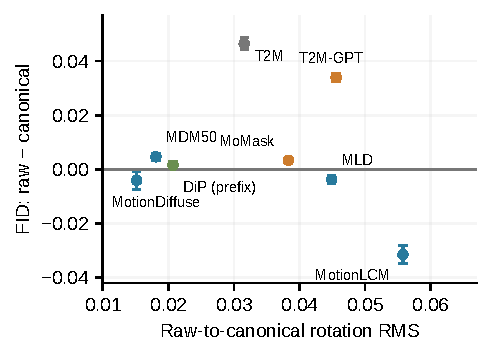
\includegraphics[width=\columnwidth]{figures/rotation_mechanism.pdf}
\caption{\textbf{Natural rotation deviations do not impose a uniform penalty.} Signed raw-minus-canonical T2M FID gaps against valid-frame raw-to-canonical rotation RMS for all eight HumanML3D release settings, with paired family-adjusted intervals. Blue: diffusion/consistency; orange: VQ; gray: VAE; green: prefix-conditioned. Family and conditioning are confounded; this is descriptive.}\label{fig:mechanism}\end{figure}

All eight HumanML3D releases appear in the mechanism analysis. Four unconditioned diffusion/consistency releases are compared descriptively with two VQ releases; T2M's VAE and prefix-conditioned DiP are shown separately. RMS is the square root of mean squared raw-to-canonical change over all valid 126 rotation values, first aggregated within each draw and then across twenty draws. It is not full-feature RMS or a norm including padding. Newly added releases use all saved outputs; earlier verified geometric records supply the original five.

Signed family means are $-0.00867$ FID for the four diffusion/consistency settings and $+0.01864$ for the two VQ settings. These are not estimates from independent model-family training replicas. T2M has the largest positive gap overall, $+0.04636$; prefix-conditioned DiP is separate. Three diffusion/consistency gaps are negative and one positive. Thus removing within-rotation noncanonicality does not uniformly favor diffusion in these releases.

Across eight release means, Spearman correlation of RMS with signed gap is $-0.095$ and with absolute gap $0.286$. Exact two-sided permutation $p$ values are 0.840 and 0.501; both adjusted values are 1.0. This small, confounded release-level analysis supplies no evidence of a monotone relation and cannot establish independence. It concerns only the exact rotation fiber and neither tests velocity/contact errors nor refutes MARDM's full representation/distribution and diffusion-training mechanism. All per-draw RMS values and original score intervals are preserved with the artifacts.

\section{Public essential-feature evaluator comparison}
\begin{table*}[t]
\centering\small
\caption{\textbf{Common-reference essential-reader comparison.} Mean embedding FID with nominal $t_{19}$ 95\% intervals over all twenty draws. The same saved real cohort is encoded separately by each reader; T2M is re-scored with this reference, which differs from its original independent-reference audit. FID scales differ across reader weights and architectures. E-CLIP FID is descriptive, not an official generation metric.}\label{tab:mardmfull}
\begin{tabular}{@{}lrrrr@{}}\toprule
Release&T2M raw&T2M $\C$&E-GRU&E-CLIP\\\midrule
MoMask&$0.0678\, [0.0651,0.0704]$&$0.0644\, [0.0618,0.0670]$&$0.0459\, [0.0432,0.0487]$&$0.0052\, [0.0050,0.0053]$\\
T2M-GPT&$0.1829\, [0.1765,0.1893]$&$0.1489\, [0.1431,0.1547]$&$0.4013\, [0.3201,0.4826]$&$0.0079\, [0.0077,0.0080]$\\
DiP (prefix)&$0.3665\, [0.3175,0.4155]$&$0.3650\, [0.3166,0.4133]$&$0.3299\, [0.2905,0.3693]$&$0.0160\, [0.0151,0.0169]$\\
MLD&$0.4446\, [0.4336,0.4556]$&$0.4483\, [0.4372,0.4595]$&$0.4269\, [0.4129,0.4410]$&$0.0166\, [0.0163,0.0168]$\\
MDM50&$0.4540\, [0.4221,0.4859]$&$0.4494\, [0.4178,0.4810]$&$0.4555\, [0.4200,0.4911]$&$0.0246\, [0.0238,0.0255]$\\
MotionLCM&$0.5740\, [0.5614,0.5867]$&$0.6055\, [0.5916,0.6194]$&$0.6125\, [0.5922,0.6329]$&$0.0188\, [0.0184,0.0191]$\\
MotionDiffuse&$0.9752\, [0.8845,1.0659]$&$0.9793\, [0.8897,1.0689]$&$1.0269\, [0.9385,1.1153]$&$0.0383\, [0.0367,0.0399]$\\
T2M&$1.3914\, [1.3648,1.4180]$&$1.3450\, [1.3181,1.3719]$&$0.9966\, [0.9720,1.0212]$&$0.0319\, [0.0316,0.0323]$\\
\bottomrule\end{tabular}\end{table*}

\begin{table}[t]
\centering\footnotesize
\caption{\textbf{Essential-only evaluation is a different remedy.} Within-reader ranks of mean embedding FID over twenty common-reference draws. Guo $\C$ retains rotations; MARDM GRU/CLIP use 67 essential features. CLIP FID is descriptive. Ranks compare these saved release settings, not published leaderboards or evaluator accuracy.}\label{tab:mardmranks}
\begin{tabular}{@{}lrrr@{}}\toprule
Release&Guo $\C$&E-GRU&E-CLIP\\\midrule
MoMask&1&1&1\\
T2M-GPT&2&3&2\\
DiP (prefix)&3&2&3\\
MLD&4&4&4\\
MDM50&5&5&6\\
MotionLCM&6&6&5\\
MotionDiffuse&7&8&8\\
T2M&8&7&7\\
\bottomrule\end{tabular}\end{table}

The public MARDM~\cite{mardm2025} checkpoint contains a 67-feature GRU reader and a motion/text Transformer contrastive reader. Both use the author normalization for root/local position features. Native layers and public states are loaded strictly. The CLIP constructor's unused visual tower is avoided using only token/position embedding placeholders; the released state then overwrites every parameter, checked bitwise before inference. No forward operation or fitted weight is replaced.

All eight saved releases and twenty original draws are evaluated without generation or training. A common saved real cohort is separately encoded by every reader. T2M scores are recomputed against the same real cohort rather than its original independent real-reference draw, so the values in \cref{tab:mardmfull} differ slightly from the original release audit. MDM, MotionDiffuse and DiP have 1,024 outputs; other releases have 4,640. DiP remains prefix-conditioned. Within each reader, rankings use twenty-draw mean embedding FID. Essential-CLIP FID is descriptive latent distance, not an official leaderboard metric, and its numerical scale cannot be compared with GRU/T2M FID.

Changing only rotation coordinates leaves the first 67 input values bitwise fixed. Native repeated forwards on the first 32 outputs of every release/draw give exactly equal essential-reader embeddings. This expected structural invariance is not an accuracy-cost test. Canonical T2M retains rotations and has the same mean ordering as raw T2M here; essential GRU changes the DiP/T2M-GPT and T2M/MotionDiffuse ordering, while essential CLIP changes MDM/MotionLCM and T2M/MotionDiffuse. Both have Kendall agreement 0.857 with canonical T2M. The ranking differences combine feature selection, architecture and different fitted weights; they cannot be attributed solely to removal of rotation redundancy or interpreted as a reliable leaderboard reversal.

All 640 saved metric cells, mean intervals and rankings are recomputed independently. Native parameter/state checks and first/last-draw inference fixtures verify the released computation. For the rotation-only sign-language representations, an essential-only input analogous to discarding HumanML3D rotations would remove all movement features. Canonicalization instead retains every represented joint rotation; its accuracy remains a separate empirical question.
